One widely used variant to deal with the before mentioned problems for Recurrent Neural Networks are LSTMs. 
These so called Long-Short-Term-Memory (LSTM) Neural Networks split the two tasks the recurrent state element \textbf{s} in basic Recurrent Neural Networks has into two layers present in each processing unit which are controlled by gates. 
Therefore these models are considered gated-architectures and the accessed memory is regulated and so is its output \citep{goldberg2017neural}.

A LSTM Neural Network unit incorporates a context layer $c$ which tries to capture the information relevant for future predictions while forgetting some of its past information. 
This layer is regulated by the forget gate and the input gate.

Additionally, the units possess a hidden state $h$ layer that gets updated by the current context state and this update is regulated by the so called output gate. Since the context state captures structural information relevant for future predictions, the hidden state can capitalize on the task of encompassing the most valuable information for the current prediction \citep{jurafsky2021}.

These additional internal mechanisms, called gates, in combination with the additional context layer are integrated to, as  \citet{embedding2020pilehvar} puts it, make the memory last longer.


\begin{figure}
    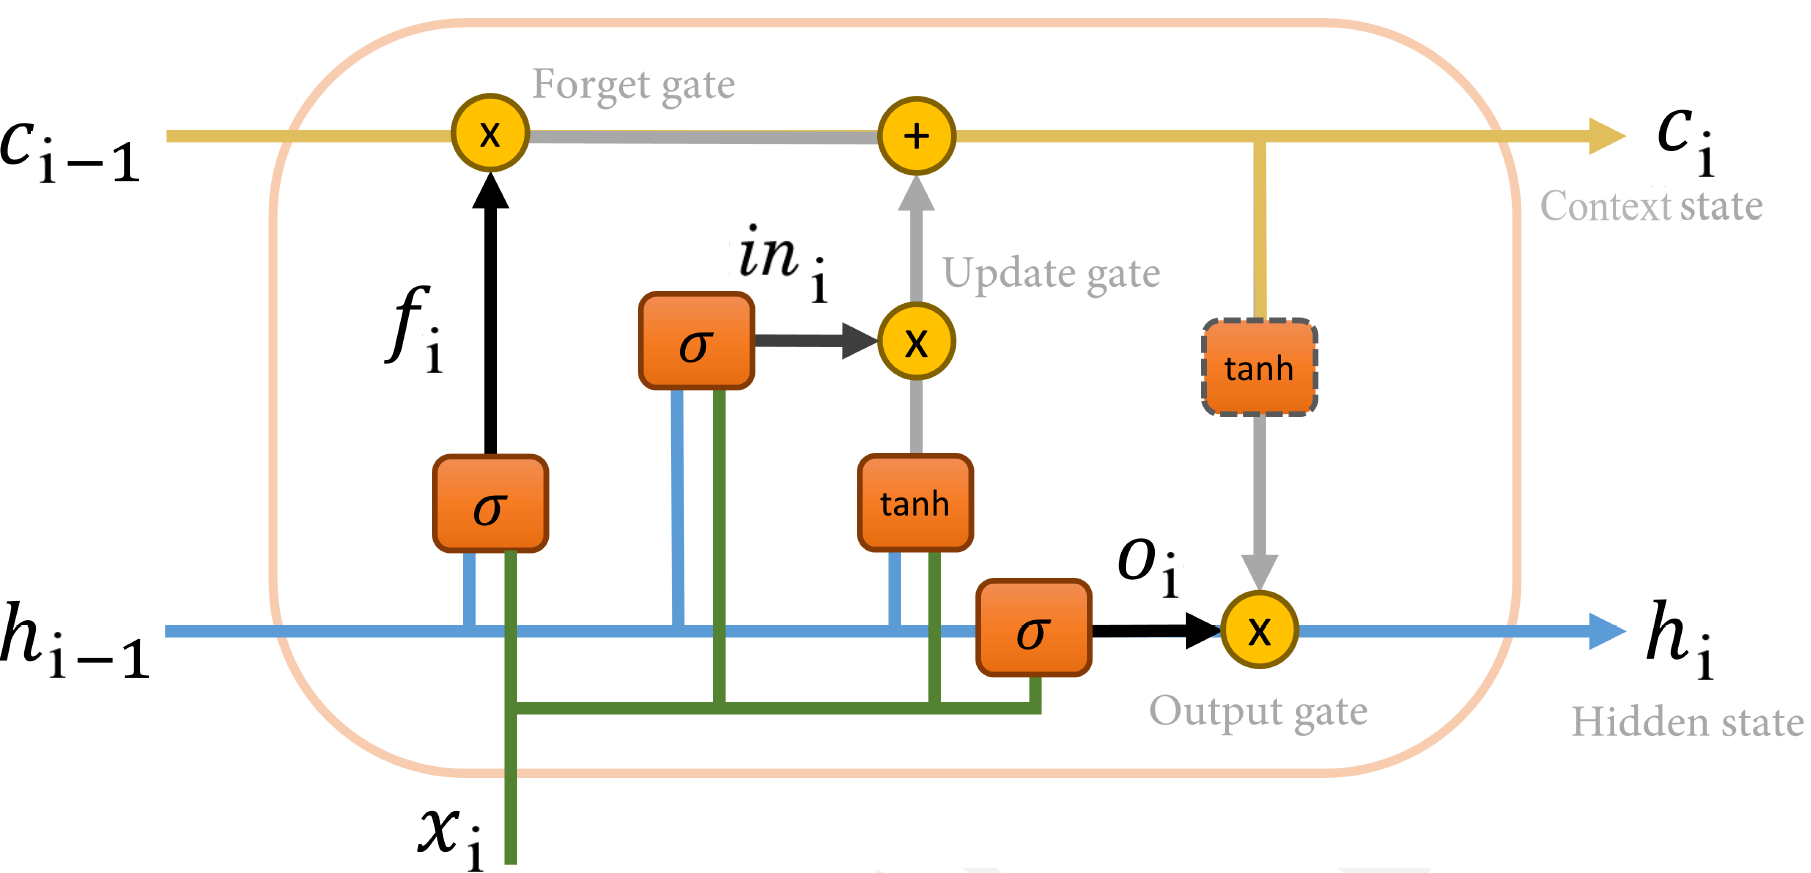
\includegraphics[width=\linewidth]{Pictures/Pilehvar_20_LSTM.png}
    \caption{Adapted and modified from \citet{embedding2020pilehvar}: Visualization of a processing unit in a LSTM. It receives the previous hidden state $h_{i-1}$, the previous context state $c_{i-1}$, the current input vector $x_i$} and produces as outputs the hidden state $h_i$ and context state $c_i$ for the current step in the sequence. The forget gate $f_i$, the input gate $in_i$ and the output gate $o_i$ are the controlling mechanisms to regulate the information flow between its inputs and outputs.
    \label{fig:LSTM}
\end{figure}

In figure \ref{fig:LSTM} the installation of an unit in a LSTM is visualised. Each unit gets fed the current input $x_i$ along with the hidden state $h_{i-1}$ and the context state $c_{i-1}$ of the calculation this unit has made for the preceding input.

\begin{equation}
\label{eq:f_gate}
    f_i = \sigma(\textbf{W}^{(x) (f)} x_i + \textbf{W}^{(h) (f)} h_{i-1} + b^{(f)})
\end{equation}

\begin{equation}
\label{eq:in_gate}
    in_i = \sigma(\textbf{W}^{(x) (in)} x_i + \textbf{W}^{(h) (in)} h_{i-1} + b^{(in)})
\end{equation}

\begin{equation}
\label{eq:o_gate}
    o_i = \sigma(\textbf{W}^{(x) (o)} x_i + \textbf{W}^{(h) (o)} h_{i-1} + b^{(o)})
\end{equation}

The forget gate, equation \ref{eq:f_gate}, has its own set of parameters which consists of weights $\textbf{W}^{(x)(f)}$ that are multiplied with the current input vector, weights $\textbf{W}^{(h)(f)}$ that are multiplied with the previous hidden state and its own bias vector $b^{(f)}$. After the multiplications with weights and the addition of its bias, the sigmoid function is used element-wise on the resulting vector. 
Therefore the output of this gate is a vector with values between 0 and 1. 

The intuition behind this procedure is that for values nearing 1 in the output of the forget gate almost all the memory of the respective value in the previous context state is retained and for values nearing 0 almost all the memory is removed.

Similarly the input gate, equation \ref{eq:in_gate}, and the output gate, equation \ref{eq:o_gate}, have their respective parameters and usage of the sigmoid function. So all gates result in vectors of values between 0 and 1 to control the flow of information. While the input gate controls what information may be incorporated of the new input, the output gate controls to what extend the information kept in the current context state propagates to the hidden state \citep{embedding2020pilehvar}.

\begin{equation}
\label{eq:cstate}
    c_i = f_i \circ c_{i-1} + in_i \circ tanh(\textbf{W}^{(x) (c)} x_i + \textbf{W}^{(h) (c)} h_{i-1} + b^{(c)})
\end{equation}

Equation \ref{eq:cstate} shows that the current context state $c_i$ is computed by the hadamard-product, the element-wise multiplication of two vectors \citep{goldberg2017neural}, of the result of the forget gate $f_i$ with the previous context state $c_{i-1}$ and the addition of new information  which is controlled by the input gate $in_i$ similarly. The informations regulated by the input gate is provided by a separate computation of the input vector $x$, previous hidden state vector $h_{i-1}$ and its own set of parameters, passed element-wise through the $tanh$ function.

Once we have the current context state $c_i$, the hidden state $h_i$ can be computed by the hadamard-product of the result of the output gate with the current state element put through the $tanh$ function. This equation can be seen in \ref{eq:hstate}. The result of this computation is also considered as the output for the unit in general.


\begin{equation}
\label{eq:hstate}
    h_i = o_i \circ tanh(c_i)
\end{equation}

\begin{equation}
\label{eq:slstm}
    s_i = R_{LSTM}(s_{i-1}, x_i) = [c_i, h_i]
\end{equation}


To summarize the equations presented in this chapter one can unite them by defining the former unspecified function $R$ for Recurrent Neural Networks presented in \ref{nn_rnn} and define the recurrent state element $s$ as the tuple of the context and hidden state as shown in equation \ref{eq:slstm}.


Finally, a major advantage these LSTM Neural Network provide is the fact that the vanishing gradient problem may be avoided since no activation function is used on track the context state takes through the LSTM cell. Therefore the error backpropagation algorithm may take place without encountering vanishing gradients as easily as in basic Recurrent Neural Networks \citep{embedding2020pilehvar}.

All the gates and computations presented in figure \ref{fig:LSTM} are encapsulated in the units, so only the context state is an additional complexity that reaches the external level of the whole neural network. This modularity is considered as the key to the power and widespread applicability of LSTMs by \citet{jurafsky2021}.